\section{Software Architecture} 

This section describes the technologies and frameworks that we used to develop our agents and how they are integrated.  We used the EISMASSim framework~\cite{behrens:2011} to communicate with the contest server, since the competition is built on Java MASSim platform and Java EISMASSim framework is distributed with the competition files.  The programming language used to develop our agents is Jason (version 1.3.8) \cite{bordini:2007}. Its concept of BDI agents provided useful resources to build our agents, like plans and intentions, which allowed us to implement the strategies and to provide our agents with long-term goals. Another advantage of Jason is its interpreter that allow us to call Java methods, which simplifies the implementation of some algorithms and enables them to run faster. These methods are integrated with our Jason agents using internal actions. More specifically we implemented two algorithms as Java methods: Dijkstra algorithm to find the best path between vertices and Breadth-First Search algorithm to locate the best area in the graph.

A blackboard was used to share and build knowledge about the environment in the form of a graph. The process to update information in the graph has a high computational cost, lasting more than one step. Therefore, to avoid losing steps, the graph is updated and shared every three steps.  The agent interaction is divided in two modes: agent-to-environment and agent-to-agent. In the first mode, in each step the EISMASSim framework receives an XML text from the server with the agents percepts, these percepts are then translated into Jason environment perceptions for our agents. This translation however does not happen when our team conquers the full map and the quantity of perception is so huge that the agents are not able to process them on time. In this case, perception is disabled and a default action (e.g. recharge) is sent back to the server. The actions of the agents are translated into text and sent to the server by EISMASSim. The Fig. \ref{arqfluxo} exemplifies how actions and percepts are exchanged. The agent-to-agent interaction uses Jason speech act based communication.  
%an XML 

\begin{figure} 
\centering 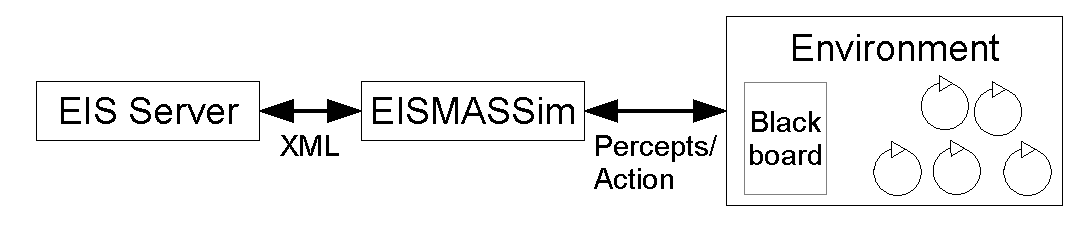
\includegraphics [width=0.9\linewidth] {./fluxo.pdf} 
\caption{Communication architecture.} \label{arqfluxo} 
\end{figure}
